\section{Supervised ML, Similarities, kNN \& Performance measurments}

\subsection{Supervised ML}
\begin{itemize}
    \item Goal: Find the best Hypothesis
    \[
    H^* = \arg \min_{H\in\mathcal{H}}\sum_{i=1}^{n}loss(x_i,y_i)
    \]
    \item Loss: 
    \[
        loss(x_i,y_i) = (H(x_i) - y_i)^2
    \]
    \item Model: \(H(x) = a + bx + cx^2 + \cdot\)
\end{itemize}
Task of the Learning Algorithem to find best parameters \(a,b,c\)(those that minimize the loss)
\subsubsection{Overfitting}
Model learns traning data but doesnt generalize well.

\subsubsection{Training and test error}
Dataset gets split in Training set and Test set (80\%/20\%)
\(error_{train}\): Error form trained model on train set

\(error_{test}\): Estimate of the true error (generalization error). Error from trained model on test set.
\subsection{kNN}
Pros:
\begin{itemize}
    \item Simple and intuitive
    \item Multiclass
    \item Interpretable 
\end{itemize}
Cons:
\begin{itemize}
    \item Curse of Dimensionality
    \item Sensitive to noise
    \item Computationally expensive for large datasets
\end{itemize}
Given training set \(X = (x_1,\text{class}_1)(x_2,\text{class}_2)\)

Given a new instance \(x_?\):
\begin{itemize}
    \item Find the k-closest examples \(x_i\) to \(x_?\) in the traning set
    \item Classify \(x_?\) based on the majority vote of \(\left\{x_{NN1},x_{NN2},\dots\right\}\)
\end{itemize}
\subsubsection{Distance and similarity measurments}
\begin{figure}[!h]
    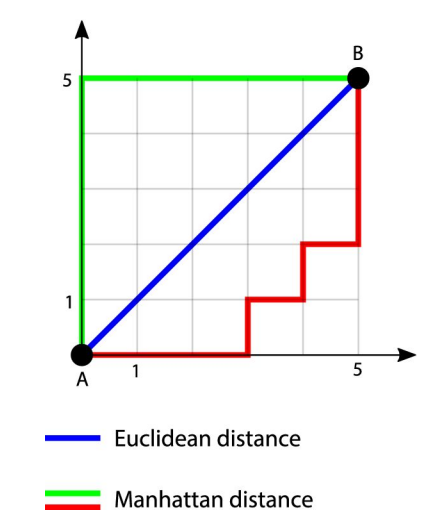
\includegraphics[width = 0.4\columnwidth]{figures/02/distances.png}
\end{figure}
Given 2 point \(\mathbf{q} = (q_1,q_2,\dots,q_n)\) and \(\mathbf{p}= (p_1,p_2,\dots,p_n)\).
\(n\) is the number of dimensions.
\subsubsection*{Euclidean Distance}
\[
d(\mathbf{q},\mathbf{p}) = \sqrt{\sum_{i=1}^{n}(q_i- p_i)}
\]
\subsubsection*{Manhatten Distance}
\[
    d(\mathbf{q},\mathbf{p}) = ||\mathbf{q}-\mathbf{p}||_1 = \sum_{i= 1}^{n}|q_i-p_i|
\]

\subsection{Finding k}
\(k_{opt} \in \{1,2,\dots,N\}\) N = \# of training samples

Extreme cases:
\begin{itemize}
    \item \(k = 1\): kNN = NN
    \item \(k = N\): Majority class
\end{itemize}
\subsection{Performance measures}
\begin{itemize}
    \item Accuracy: \#corr / \#all = (TP + TN) / (TP + FN + FP + TN)
    \item Error: \#wrong / \#all = 1 -  Accuracy
    \item Recall,Sensitivity: TP /(TP + FN), How many relevant samples are correctly detected
    
    \item Specificity: TN/(TN + FP)
    \item Precision: TP/(TP + FP), How many detected samples are relevant
    \item F1 score: 2 \(\cdot\) Precision \(\cdot\) Recall / ( Precision + Recall)
\end{itemize}

\subsubsection{ROC (Receiver Operating Characteristic) curve}
TPR, FPR, to find best threshold.
\begin{figure}[!h]
    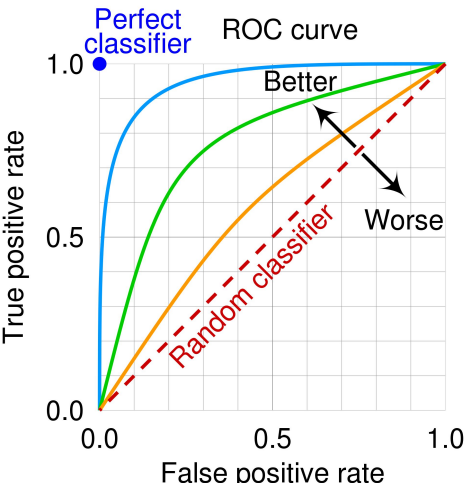
\includegraphics[width = 0.45\columnwidth]{figures/02/ROC.png}
    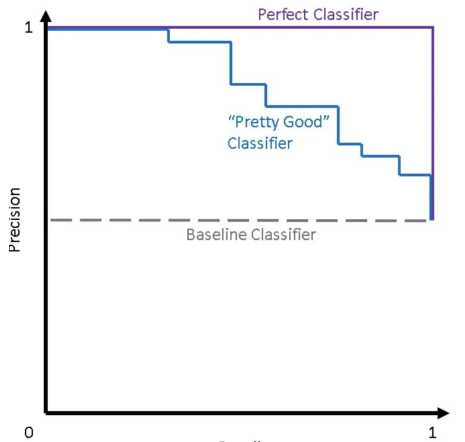
\includegraphics[width =0.45 \columnwidth]{figures/02/PRC.png}
\end{figure}

\subsubsection{PRC(Precision-Recall Curve)}
Precision, Recall, to find best threshold.

